\documentclass{article}

% Language setting
% Replace `english' with e.g. `spanish' to change the document language
\usepackage[spanish,mexico]{babel}

% Set page size and margins
% Replace `letterpaper' with `a4paper' for UK/EU standard size
\usepackage{caption}
\usepackage{subcaption}

\usepackage[letterpaper,top=2cm,bottom=2cm,left=3cm,right=3cm,marginparwidth=1.75cm]{geometry}

% Useful packages
\usepackage{amsmath}
\usepackage{graphicx}
\usepackage[colorlinks=true, allcolors=blue]{hyperref}


\title{Avance de tesis}
\author{Erick Felipe Serrato Garcia \\ Informe de la semana 5, trimestre 23-P}

\begin{document}
\maketitle

\section{Introducción}

El cancer es uno de los temas médicos más relevantes en la actualidad debido al riesgo que este presenta en todos los sectores de la población, en caso de que no se detecte a tiempo puede llegar a ser muy dificil de tratar e inclusive solo dar tratamiento para extender la vida del paciente un poco más.

Cuando una célula envejece y pierde su capacidad de dividirse termina su ciclo de vida, las células cancerígenas son células anomalas que presentan mutaciones en los genes que regulan el ciclo celular, por ello pueden crecer descontroladamente hasta formar densidades grandes de ellas y posteriormente diseminarse a otras partes del cuerpo.

El cuerpo humano puede defenderse de diferentes amenazas, desde las que ingresan del exterior hasta las que se producen en el interior, en el caso de las células cancerigenas, si el cuerpo humano se encuentra saludable (entre otros factores) puede erradicar y/o contener la enfermedad. A la interacción en la que las células defensoras eliminan a las anomalas se le llama citotoxicidad.

Cuando el sistema inmune detecta una anomalía, envia a las células llamadas "natural killers" que es un tipo de glóbulo blanco que puede matar células tumorales, células infectadas por virus o cualquier cosa que consideren anomala, estas no siempre tienen exito en su misión, cuando eso sucede, el sistema inmune envía a los lifocitos T o células T las cuales identifican a las células infectadas y las eliminan mediante un proceso llamado aptosis y posteriormente otras células "limpiadoras" llamadas macrofagos terminan de limpiar los restos.

\subsection{Efecto Allee}

La interacción entre células del sistema inmune y cancerigenas puede explicarse de manera general como una dinámica de poblaciones entre presas y predadores, en la naturaleza si una densidad de población es demasiado baja y continua bajando se tiene una tasa de crecimiento negativa, tenemos otro caso en el cual la tasa de crecimiento es baja pero positiva, esto puede ser modelado mediante el efecto Allee fuerte y débil respectivamente, esto podemos visualizarlo en la Figura \ref{fig:allees}.


\begin{figure}[ht]
    \centering
    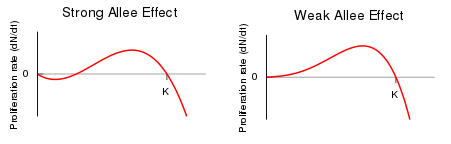
\includegraphics[width=0.6\textwidth]{images/Allee.png}
    \caption{Efecto Allee débil y fuerte}
    \label{fig:allees}
\end{figure}

En el efecto Allee débil (ecuación \ref{eqn:weak_allee}) la tasa de crecimiento aumenta con la densidad de población y permanece positiva, en el efecto fuerte \ref{eqn:strong_allee}, se tiene un umbral poblacional por debajo del cual la población decrece hasta llegar a la extinción.

\begin{equation}
    \frac{d x}{ dt} = r x (1 - \frac{x}{k})(1- \frac{A+ c}{x + c})
    \label{eqn:strong_allee}
\end{equation}

El caso débil es cuando $A\leq 0$, si consideramos $A=0$ y se obtiene:

\begin{equation}
    \frac{d x}{ dt} = r x (1 - \frac{x}{k})(\frac{x}{x + c})
    \label{eqn:weak_allee}
\end{equation}

En el año 2020 Marcello Delitala y colaboradores\cite{Marcello2020} publicarón un artículo que examina críticamente la aplicabilidad y las implicaciones del efecto Allee en el contexto de la biología del cáncer y su impacto potencial en la evolución del cáncer y las estrategias terapéuticas. Este artículo profundiza en la cuestión fundamental de si el efecto Allee, un concepto típicamente asociado con la dinámica ecológica y poblacional, tiene relevancia en el campo de la investigación del cáncer. Explica que este concepto, si bien se aplica tradicionalmente a contextos ecológicos, puede tener implicaciones inexploradas en la comprensión de la biología del cáncer, donde las poblaciones celulares se comportan de manera que se asemejan a la dinámica poblacional. Los autores detallan los métodos de investigación empleados en esta investigación, que abarcan experimentos in vitro e in vivo, modelos matemáticos y análisis de datos clínicos. Estos enfoques fueron diseñados para dilucidar si las poblaciones de células cancerosas exhiben comportamientos consistentes con el efecto Allee. El artículo presenta una recopilación sólida de resultados que demuestran que el efecto Allee es realmente relevante en el contexto de la biología del cáncer. Revela que las poblaciones de células cancerosas pueden exhibir una dinámica de crecimiento dependiente de la densidad, con tasas de crecimiento que se desaceleran con densidades celulares bajas. Estos hallazgos sugieren que los principios de los efectos ecológicos de Allee pueden aplicarse para comprender la evolución del cáncer.

Consideremos profundizar en la dinámica de las poblaciones de células cancerosas en bajas densidades, contrastando el modelo de crecimiento exponencial y considerando la presencia de un efecto Allee.

Kaitlyn y colaboradores\cite{Kaitlyn1782019} publicarón un trabajo relacionado con efecto Allee para una población de células a densidades bajas, detallan los métodos experimentales y computacionales utilizados en este estudio, incluidas técnicas de cultivo celular, recopilación de datos y modelado matemático. Destacan el enfoque riguroso adoptado para evaluar con precisión el crecimiento de las células cancerosas en condiciones controladas. El artículo presenta resultados convincentes que indican que las poblaciones de células cancerosas en bajas densidades no se ajustan al modelo de crecimiento exponencial esperado. En cambio, los datos muestran desviaciones que son propias de un efecto Allee, donde las tasas de crecimiento se desaceleran en densidades de población bajas debido a varios factores, como recursos limitados y menores interacciones cooperativas entre células. Se proponen posibles mecanismos detrás del efecto Allee observado en poblaciones de células cancerosas, como limitaciones de nutrientes, alteraciones de la señalización e interacciones entre células. La discusión también aborda la importancia potencial del efecto Allee para las estrategias de tratamiento del cáncer, lo que sugiere que los enfoques terapéuticos dirigidos a poblaciones de baja densidad pueden producir resultados prometedores.

La señalización autocrina es un mecanismo que permite a las células controlar y regular sus propias funciones. Por ejemplo, una célula puede secretar una molécula de señalización autocrina para estimular su propio crecimiento, diferenciación o supervivencia en respuesta a condiciones ambientales cambiantes o a estímulos internos. En el año 2022 Gerlee y colaboradores 
publicaron un artículo \cite{Gerlee032022} que  explora el papel de la señalización autocrina en la manifestación de los efectos Allee dentro de las poblaciones de células cancerosas. Este estudio, basado en el ámbito de la biología celular y la investigación del cáncer, revela un mecanismo novedoso que arroja luz sobre la dinámica de la progresión del cáncer, con posibles implicaciones para las estrategias terapéuticas y los resultados del tratamiento. Los autores describen exhaustivamente los métodos experimentales y computacionales empleados en su investigación, incluidas técnicas de cultivo celular, adquisición de datos y modelado matemático. Se presta especial atención al diseño meticuloso de experimentos para explicar el papel de la señalización autocrina en el crecimiento de las células cancerosas. Los datos indican que las células exhiben un mayor comportamiento cooperativo y tasas de crecimiento cuando la señalización autocrina está activa, lo que puede conducir a una proliferación acelerada en densidades celulares bajas.Además, el artículo analiza las posibles consecuencias de estos descubrimientos para las estrategias de tratamiento del cáncer. Sugiere que las intervenciones dirigidas a las vías de señalización autocrina pueden representar una vía prometedora para controlar la progresión del cáncer y mejorar los resultados terapéuticos.




\subsection{Complejo MHC y su importancia en el cancer}
La relación entre las células asesinas naturales (NK-Natural Killers), las células T y el complejo MHC gira principalmente en torno al reconocimiento de antígenos y la respuesta inmune. Las células NK no dependen del complejo MHC para su activación, principalmente reconocen y se dirigen a células que han alterado o reducido la expresión del MHC de clase I, lo que puede ser un signo de infección o malignidad. Las células T, por otro lado, tienen receptores (receptores de células T o TCR) que interactúan con las moléculas MHC presentadoras de antígenos. Las células T CD8+ reconocen antígenos presentados por moléculas del MHC de clase I, mientras que las células T CD4+ reconocen antígenos presentados por moléculas del MHC de clase II. Las moléculas del MHC desempeñan un papel fundamental en la presentación de antígenos a las células T, lo que permite a las células T distinguir entre antígenos propios y no propios y desencadenar respuestas inmunitarias específicas.

En resumen, las células NK, las células T (CD8+ y CD4+) y el complejo MHC son componentes integrales del sistema inmunitario, cada uno con funciones distintas en la vigilancia inmunitaria, el reconocimiento de antígenos y la respuesta inmunitaria. Las células NK no dependen del MHC para su activación y se dirigen a células con expresión alterada del MHC, mientras que las células T reconocen antígenos presentados por las moléculas del MHC en el contexto de la inmunidad adaptativa\cite{Jiang2019}. (Fígura \ref{fig:mhc}).

\begin{figure}[ht]
    \centering
    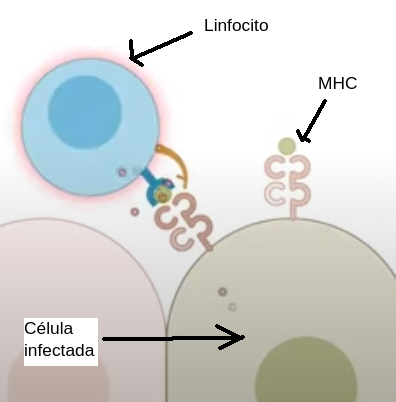
\includegraphics[width=0.4\textwidth]{images/mhc.png}
    \caption{Interacción de los linfocitos y células infectadas mediante el complejo MHC}
    \label{fig:mhc}
\end{figure}

El problema del crecimiento aberrante en la densidad de células cancerígenas es que las células infectadas pierden la capacidad de activar el MHC, por lo que no pueden ser identificadas y por lo tanto destruidas por las células T. En este punto nos preguntamos ¿si pudiesemos controlar la regulación del MHC disminuiría la densidad de células cancerigenas? la respuesta es que sí. En el año 2020 Annelisa M. Cornel y colaboradores\cite{Cornel072020} públicaron un artículo en el qué destacan que las células cancerosas a menudo emplean mecanismos para regular negativamente la expresión del MHC Clase I, escapando así de la vigilancia inmune, investigan a fondo los mecanismos responsables de la regulación negativa del MHC Clase I en el cáncer, incluidas las alteraciones genéticas, las modificaciones epigenéticas y la interferencia con el procesamiento y la presentación de antígenos. Proporcionan información sobre las diversas estrategias utilizadas por las células cancerosas para evadir el reconocimiento inmunológico, en resumen, proporcionan un análisis de los mecanismos que sustentan la regulación negativa del MHC de clase I en el cáncer y presentan posibles vías terapéuticas para la inmunoterapia, de hecho mencionan que existen terapias  aprobadas por la FDA.

Si bién lo anterior tiene un contexto biológico, necesitamos destacar la intención de utilizar herramientas de el campo de las ciencias físicas para abordar esta problemática. En el año 2016 Augusto Gonzalez \cite{Gonzalez2016} y en el año 2018 Qianqian Zheng y colaboradores \cite{Zheng2018} publicarón trabajos similares en los que profundizan en la intersección de la teoría del control y la inmunología, arrojando luz sobre la aplicación de modelos matemáticos para comprender la dinámica de la respuesta del sistema inmunológico al cáncer, estos estudios introducen modelos matemáticos que representan la dinámica de las interacciones del sistema inmunológico con las células cancerosas y abarcan componentes como células inmunes, crecimiento tumoral e intervenciones terapéuticas. Consideremos el potencial de la teoría del control matemático para avanzar en el campo de la medicina personalizada, al adaptar las estrategias de tratamiento en función de las características individuales de los pacientes, se pueden diseñar terapias contra el cáncer más efectivas.


 \newpage



\section{Modelo propuesto}

Del capítulo anterior, a densidades bajas, el cancer no tiene un crecimiento exponencial, esto debido a que las celulas inmunitarias del cuerpo humano compiten con el cancer para eliminarlo, es decir, se comportan como presas y depredadores.


Consideremos un entorno en el cual interactuan 3 especies, el cancer, células sanas y el sistema inmune. Sabemos que el cancer compite por los recursos y el espacio con las células sanas, por otra parte el sistema inmune si caza a a las células cangerigenas, por ello consideremos la siguiente tabla:

\begin{table}[h]
\begin{center}
\begin{tabular}{ | c | c | c | c | }
\hline  & Con $C$ & Con $S$ & Con $I$ \\ \hline
Interaccion de $C$ & $r_c C (\frac{C}{a} - 1)(1-\frac{C}{k_c})$ & $-\alpha CS$ & $-\beta CI$  \\ \hline
Interaccion de $S$ & $-\gamma CS$ & $r_s S (1 - \frac{S}{k_s})$  & $\delta SI$  \\ \hline
Interaccion de $I$ & $\eta C I$ &   & $r_i I(1-\frac{I}{k_i})$  \\ \hline

\end{tabular}
\end{center}
\end{table}
 
En donde   $C$ es el cancer, $S$ son las células sanas e $I$ es el sistema inmune. Como mencionamos en la sección anterior en la interaccion del cancer $C$ consigo mismo es un modelo del efecto Alle, para el caso de las células sanas $S$ y el sistema unmune $I$ consideramos una interaccion consigo mismos mediante un modelo logístico, para los otros casos, por ejemplo la interacción de $C$ con $S$  tenemos $-\alpha CS$, lo que significa que se tendrá una perdida en la cantidad de cancer si las células sanas comienzan a recuperar su territorio, esta lógica aplica para las otras interacciones lineales con signo positivo. En la interacción del sistema inmune $I$ con el cancer $C$ se esperaría que si se tiene un aumento de células cancerigenas se tenga una respuesta en el crecimiento de células inmunitarias, por ello es positivo el signo $\eta C I$, este argumento aplica para las demás interacciones lineales con signo positivo.


con ello podemos escribir el siguiente sistema de ecuaciones diferenciales ordinarias:

\begin{equation}
    \frac{dC}{dt} =  r_c C (\frac{C}{a} - 1)(1-\frac{C}{k_c}) - \alpha CS - \beta CI,
    \label{eqn:cancer_dynamic}
\end{equation}

\begin{equation}
    \frac{dS}{dt} = r_s S (1 - \frac{S}{k_s})  - \gamma CS + \delta SI,
    \label{eqn:sano_dynamic}
\end{equation}


\begin{equation}
    \frac{dI}{dt} = r_i I(1-\frac{I}{k_i}) + \eta C I.
    \label{eqn:inmune_dynamic}
\end{equation}


Analizando los elementos de la diagonal de le ecuacion consideremos el término asociado el cancer $C$ mediante el modelo del efecto Allee efecto Allee $g(C) = r_c C (\frac{C}{a} - 1)(1-\frac{C}{k_c})$, en donde $0<h<r$ corresponde al efecto Allee fuerte y $r<0$,  $h>0>r$ es el efecto débil y que al ser una ecuación cúbica tiene valores nulos para $C=0$, $C=r$ y $C=h$, podemos visualizar las curvas en la figura \ref{fig:allee_plots}

\begin{figure}[ht]
 \centering
  {
   \label{fig:strong_allee}
a)    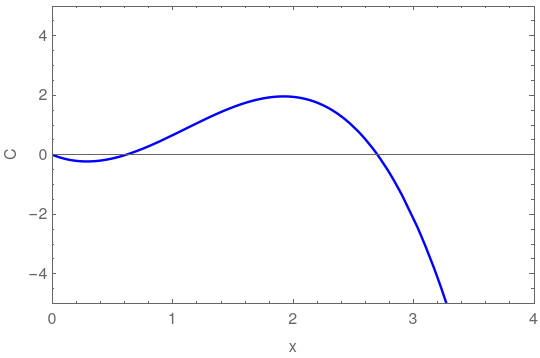
\includegraphics[width=0.45\textwidth]{images/strong_allee.png}}
  {
   \label{fig:weak_allee}
b)    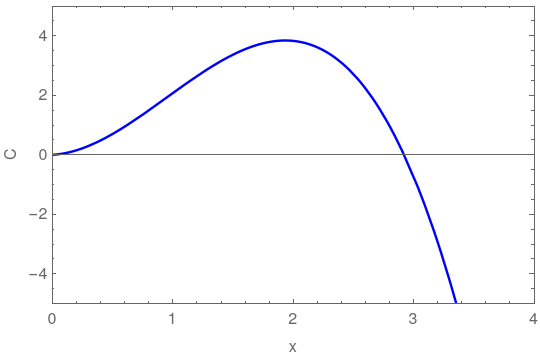
\includegraphics[width=0.45\textwidth]{images/allee_weak.png}}
  
 \caption{En $a)$ tenemos el efecto Alle fuerte para $r=2.7$ y $h=0.61$, en $b)$ tenemos el efecto débil con $r=-0.08$ y $h=2.92$}
 \label{fig:allee_plots}
\end{figure}


Para el caso de las células sanas $S$, consideramos un modelo logístico $r_s S (1 - \frac{S}{k_s})$. 

Para el sistema inmune $S$, consideramos un modelo logístico $r_i I(1-\frac{I}{k_i})$, este tiene valores nulos cuando $I=0$ y cuando $I=k_i$ es en donde la cantidad de individuos tiende a un valor constante.

\begin{figure}[ht]
    \centering
    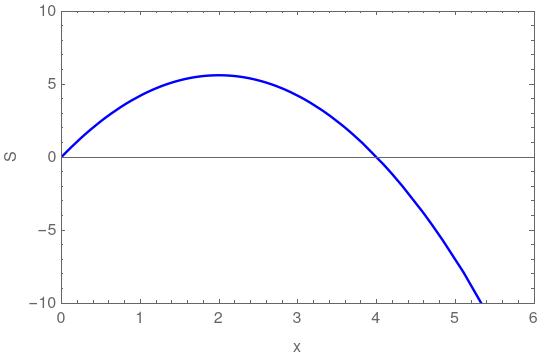
\includegraphics[width=0.5\textwidth]{images/logistic.png}
    \caption{Modelo logístico que modela la producción de céluas inmunitarias $S$, con $r_i=5.6 $ y $k_i=4$}
    \label{fig:logistic}
\end{figure}

\subsection{Escalamiento de ecuaciones diferenciales}
La finalidad de la presente sección consta de encontrar la manera de obtener un modelo lo más simple posible, el escalamiento ayuda a reducir el número de parámetros independientes, por lo que, resolver el modelo analítica o numéricamente resulta ser mas sencillo.

De las ecuaciones \ref{eqn:cancer_dynamic}, \ref{eqn:sano_dynamic}, \ref{eqn:inmune_dynamic} consideremos el cambio de variable $c=\frac{C}{k_c}$,  $s=\frac{S}{k_s}$, $i=\frac{I}{k_i}$ y $t = \frac{a}{k_c r_c} \tau $ resolviendo obtenemos:

\begin{equation}
    \frac{dc}{d \tau} =  c (c - a')(1-c) - \alpha' cs - \beta' i c,
    \label{eqn:cancer_dynamic_escalado}
\end{equation}

\begin{equation}
    \frac{ds}{d \tau} = r_s ' s (1 - s)  - \gamma' cs + \delta' si,
    \label{eqn:sano_dynamic_escalado}
\end{equation}


\begin{equation}
    \frac{di}{d\tau} = r_i ' i(1-i) + \eta' ci.
    \label{eqn:inmune_dynamic_escalado}
\end{equation}

En donde $a' = \frac{a}{k_c}$, $\alpha'= \alpha k_s$, $\beta'=\beta k_i$, $r_s'= \frac{a r_s}{k_c r_c}$, $\gamma'=\frac{a \gamma}{r_c}$, $\delta' = \frac{a \delta}{r_c k_c}$, $r_i' = \frac{a r_i}{r_c k_c}$ y $\eta' = \frac{a \eta}{r_c k_c}$

\subsection{Estados estacionarios y nulclinas}
La finalidad del presente capítulo es describir el comportamiento de nuestro modelo de ecuaciones diferenciales, en los estados estacionarios, además clasificar esos estados estacionarios depende si son estados estables o inestables así como entender la dinámica alrededor de estos estados, por ello consideramos también tomar la ruta de estudiar las nulclinas.

Los estados estacionarios se encuentran cuando se cumple que las ecuaciones \ref{eqn:cancer_dynamic_escalado}, \ref{eqn:sano_dynamic_escalado} y \ref{eqn:inmune_dynamic_escalado} no varian temporal ni espacialmente, es decir:

\begin{equation}
    c (c - a')(1-c) - \alpha' cs - \beta' i c = 0,
    \label{eqn:cancer_dynamic_escalado_2}
\end{equation}

\begin{equation}
     s (1 - s)  - \gamma'' cs + \delta'' si = 0,
    \label{eqn:sano_dynamic_escalado_2}
\end{equation}


\begin{equation}
    i(1-i) + \eta'' ci = 0.
    \label{eqn:inmune_dynamic_escalado_2}
\end{equation}

En donde $\gamma'' = \frac{\gamma k_c}{r_s}$,  $\delta'' = \frac{\delta}{r_s}$ y $\eta'' = \frac{\eta}{r_i}$,  las ecuaciones \ref{eqn:cancer_dynamic_escalado_2}, \ref{eqn:sano_dynamic_escalado_2} y \ref{eqn:inmune_dynamic_escalado_2} se cumplen cuando $c=0$, $s=0$ e $i=0$ y cuando 

\begin{equation}
    (c - a')(1-c) - \alpha' s - \beta' i  = 0,
    \label{eqn:cancer_dynamic_escalado_3}
\end{equation}

\begin{equation}
    (1 - s)  - \gamma'' c + \delta'' i = 0,
    \label{eqn:sano_dynamic_escalado_3}
\end{equation}


\begin{equation}
    (1-i) + \eta'' c = 0.
    \label{eqn:inmune_dynamic_escalado_3}
\end{equation}

de la ecuación  \ref{eqn:inmune_dynamic_escalado_3} podemos despejar

\begin{equation}
    c =  \frac{ i-1}{\eta},
    \label{eqn:inmune_dynamic_escalado_4}
\end{equation}

Sustituyendo \ref{eqn:inmune_dynamic_escalado_4} en \ref{eqn:cancer_dynamic_escalado_3} y despejando tendremos:

\begin{equation}
 F_1 (s,i) = -s \alpha' - i\beta' - \frac{(-1+i-\eta'')(-1+i -a \eta'')}{(\eta'')^2}  = 0
    \label{eqn:sol_s1}
\end{equation}


De la ecuación \ref{eqn:sol_s1} despejamos a $s$ lo que nos dá:

\begin{equation}
    s_a(i) = -\frac{a' (\eta'') ^2+a' \eta'' +\eta'' +1}{\alpha'  (\eta'') ^2}+\frac{ \left(a' \eta'' -\beta'  (\eta'') ^2+\eta''
   +2\right)}{\alpha'  (\eta'') ^2}i-\frac{i^2}{\alpha'  (\eta'') ^2}
   \label{eqn:sol_s11}
\end{equation}


Sustituyendo \ref{eqn:inmune_dynamic_escalado_4} en \ref{eqn:sano_dynamic_escalado_3} y despejando tendremos:

\begin{equation}
    F2(s,i) = -\delta''  i-\frac{\gamma''  (i-1)}{\eta }-s+1 = 0
    \label{eqn:sol_s22}
\end{equation}

y nuevamente, despejando a $s$, tenemos:

\begin{equation}
    s_b(i) = -\frac{i (\gamma'' +\delta''  \eta'' )}{\eta'' }+\frac{\eta'' +\gamma''  }{\eta'' }
    \label{eqn:sol_s2}
\end{equation}


Desarrollando el proceso algebraico caemos en el hecho de que es posible obtener ciertos valores $(s_j,c_j,i_j)$ que solo dependen de los parametros $\gamma,\eta,\beta,a,\alpha,\delta, r_i,r_s$ que es lo que conocemos como estados estacionarios, en este caso tenemos 3 puntos que satisfacen a estas ecuaciones

\begin{equation}
   P_1 = (c_1, s_1, i_1)    
\end{equation}

\begin{equation}
    P_2 = (c_2, s_2, i_2)
\end{equation}

\begin{equation}
    P_3 = (0, 0, 0)
\end{equation}

La intersección en las ecuaciones \ref{eqn:sol_s1} y \ref{eqn:sol_s22} pueden tener valores positivos y negativos, sin embargo, las densidades de población no tienen sentido para valores negativos por lo que además de buscar los puntos $P_1$ y $P_2$, también debe cumplirse que sean positivos, en la figura \ref{fig:nullclines} podemos observar algunos de los valores para los parámetros los cuales se cumplen estas condiciones.


\begin{figure}[h]
	\centering
	\begin{subfigure}{0.4\linewidth}
		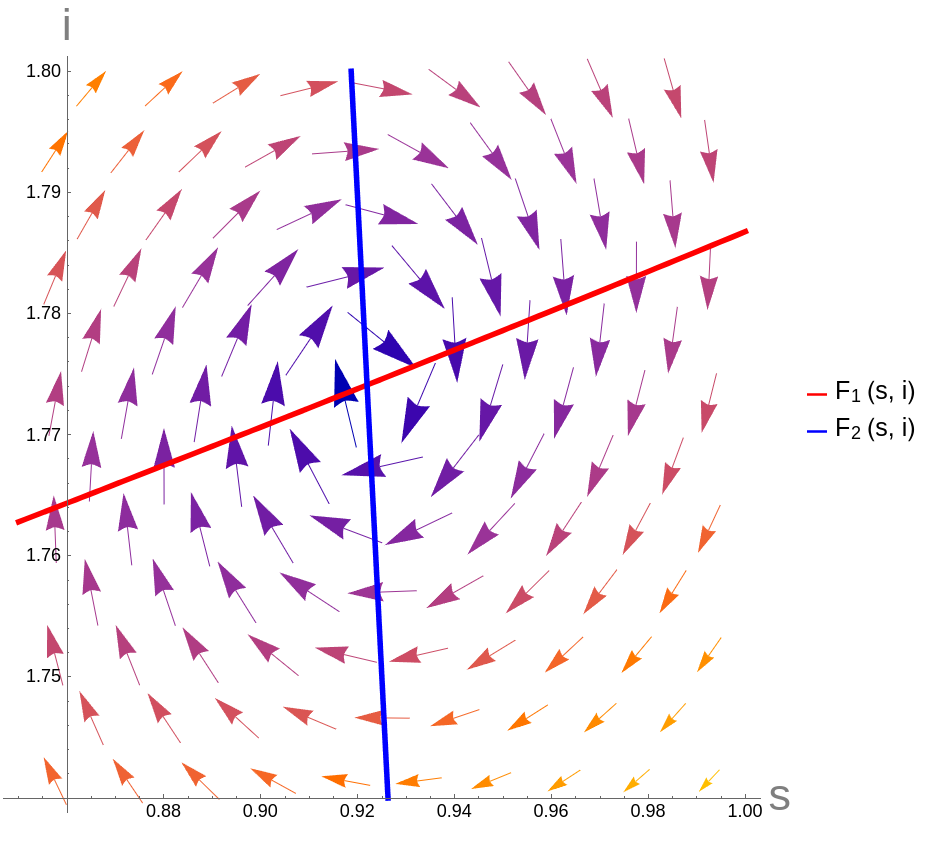
\includegraphics[width=\linewidth]{images/nullclines_1.png}
		\caption{$P1$ Nodo neutral estable}
		\label{fig:subfigA}
	\end{subfigure}
        \hspace{0.2cm}
	\begin{subfigure}{0.4\linewidth}
		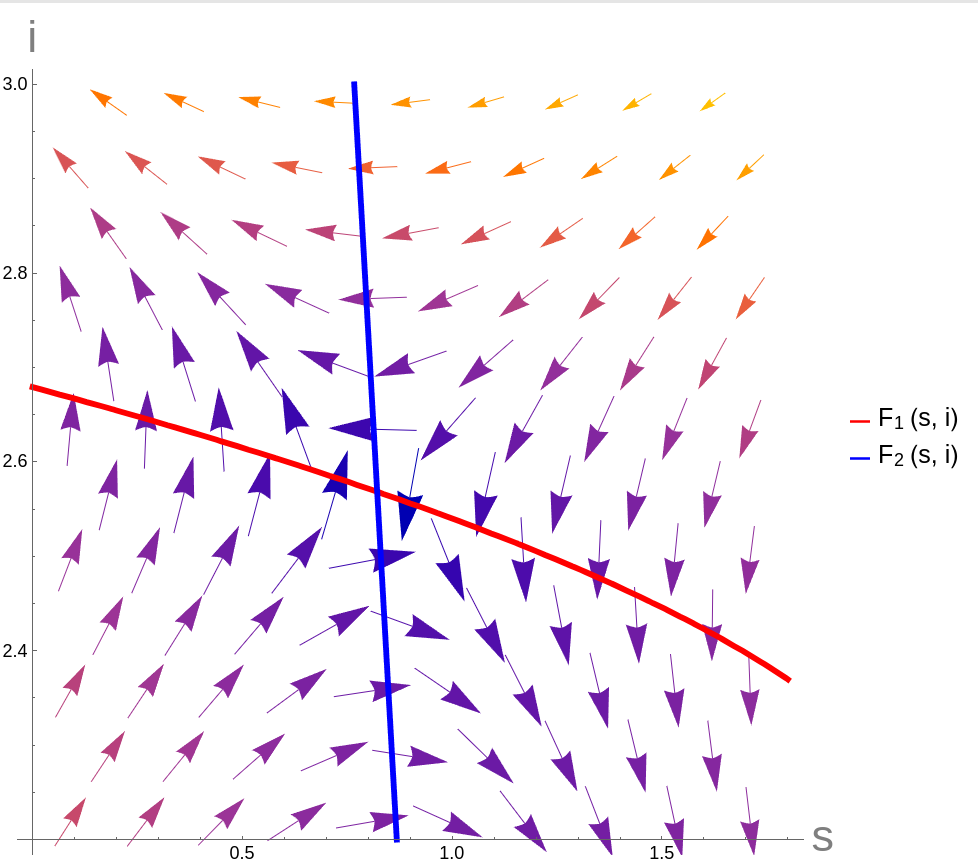
\includegraphics[width=\linewidth]{images/nullclines_2.png}
		\caption{$P2$ Nodo silla inestable}
		\label{fig:subfigB}
	\end{subfigure}
	\caption{Representación gráfica de las ecuaciones $F_1(s,i)$ (azul) y $F_2(s,i)$ (rojo), para los valor es de $a'=2.83$, $\alpha'=0.33$, $\beta'=0.06$, $\gamma''=0.054$, $\delta''=0.012$, $\eta''=0.365$, $r_i=0.595$, $r_s=0.6$ con $P_1(c,s,i)=(1.261, 0.921, 1.774)$ y $P_2(c,s,i)=(2.556, 0.821, 2.568)$ }
	\label{fig:nullclines}
\end{figure}



\newpage

\subsection{Solución a EDO en estados estacionarios}


\begin{figure}[ht]
    \centering
    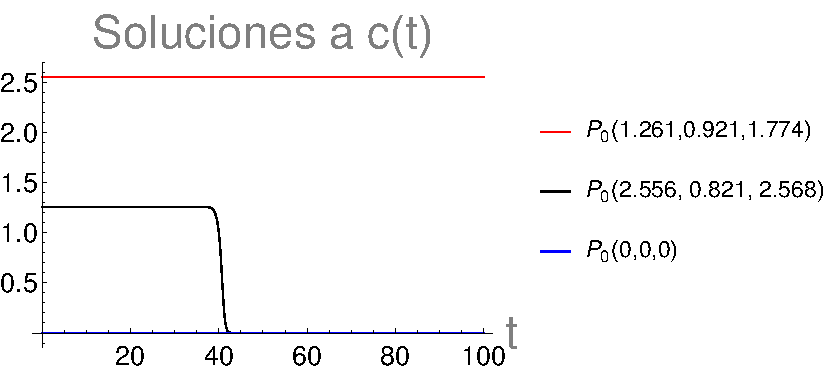
\includegraphics[width=0.7\textwidth]{images/solucion_c.pdf}
    \caption{Solución edo c}
    \label{fig:sol_edo_c}
\end{figure}


\begin{figure}[ht]
    \centering
    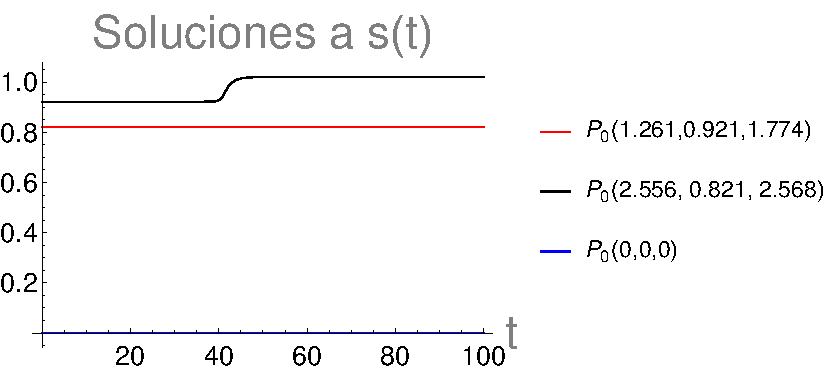
\includegraphics[width=0.7\textwidth]{images/solucion_s.pdf}
    \caption{Solución EDO s}
    \label{fig:sol_edo_s}
\end{figure}


\begin{figure}[ht]
    \centering
    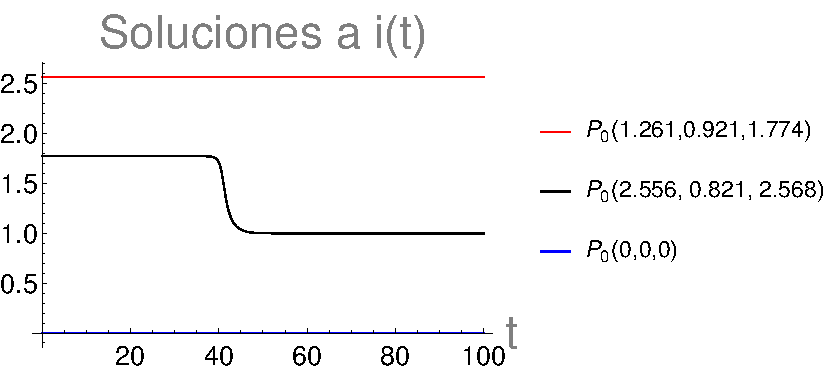
\includegraphics[width=0.7\textwidth]{images/solucion_i.pdf}
    \caption{Solución EDO i}
    \label{fig:sol_edo_i}
\end{figure}


\newpage
\subsection{Analisis de estabilidad lineal}
Si bien contamos con un modelo de ecuaciones diferenciales, hasta ahora conocemos las soluciones en los estados estacionarios, una pregunta interesante sería, ¿como interactua el cancer, sistema inmune y células sanas en un organo, en la piel, etc etc?. Bajo esta pregunta proponemos llevar a las ecuaciones diferenciales a un sistema de ecuaciones diferenciales parciales con dependencia espacial al modificarlas toman la forma de un sistema reacción difusión agregando $D_c \nabla ^2 c$, $D_s \nabla ^2 s$, $D_i \nabla ^2 i$ en donde $\nabla ^2$ es el laplaciano y $D_i$, $D_s$ y $D_c$ son los coheficientes de difusión.

Ahora consideremos el sistema de ecuaciones \ref{eqn:cancer_dynamic_escalado}, \ref{eqn:sano_dynamic_escalado} y \ref{eqn:inmune_dynamic_escalado} con dependencia espacial

\begin{equation}
    \frac{\partial c}{\partial \tau} = D_c \nabla ^2 c +  c (c - a')(1-c) - \alpha' cs - \beta' i c,
    \label{eqn:cancer_dynamict_escalado}
\end{equation}

\begin{equation}
    \frac{\partial s}{\partial \tau} = D_s \nabla ^2 s + r_s ' s (1 - s)  - \gamma' cs + \delta' si,
    \label{eqn:sano_dynamict_escalado}
\end{equation}


\begin{equation}
    \frac{\partial i}{\partial \tau} = D_i \nabla ^2 i + r_i ' i(1-i) + \eta' ci.
    \label{eqn:inmune_dynamict_escalado}
\end{equation}

\begin{figure}[ht]
    \centering
    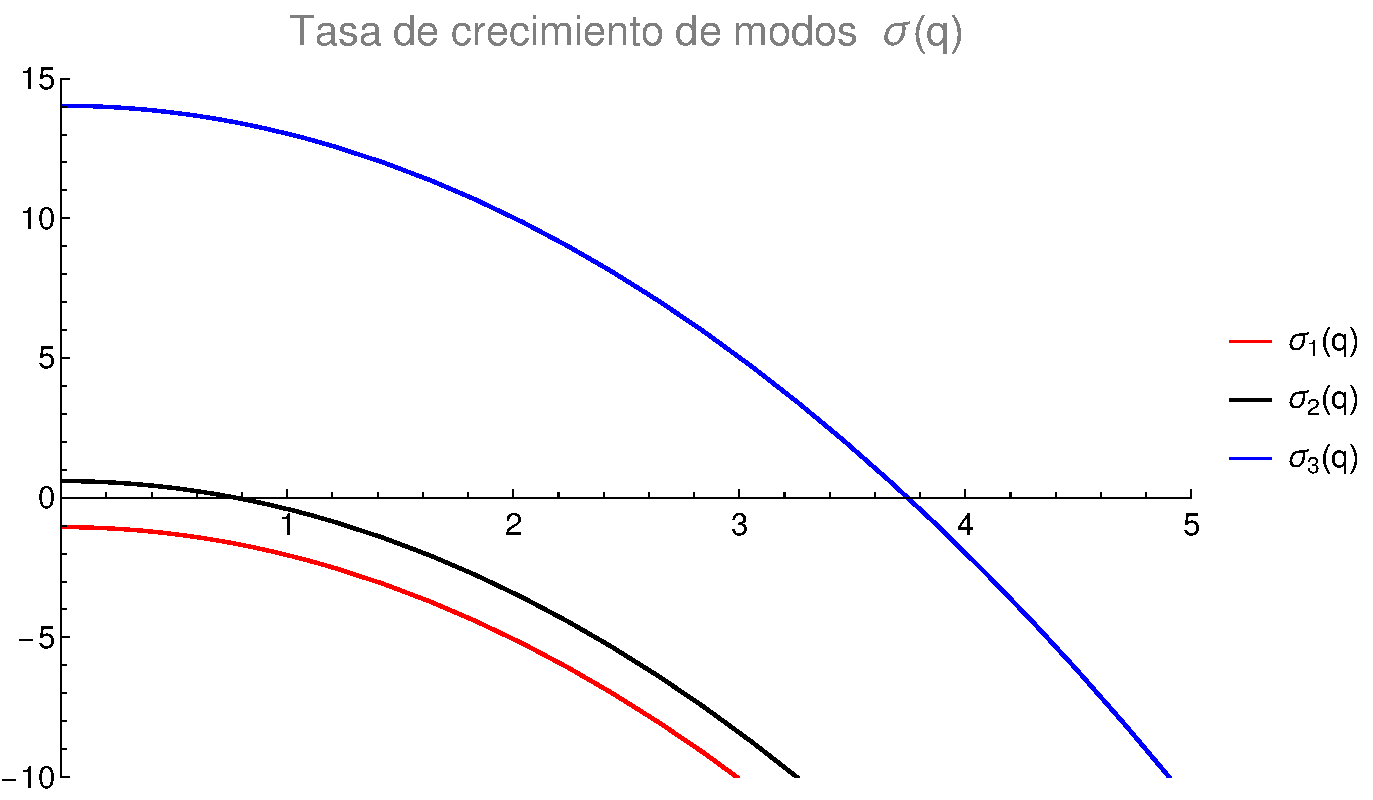
\includegraphics[width=0.6\textwidth]{images/estabilidad_p1.pdf}
    \caption{Estabilidad $P_1$}
    \label{fig:estabilidad_p1}
\end{figure}


\begin{figure}[ht]
    \centering
    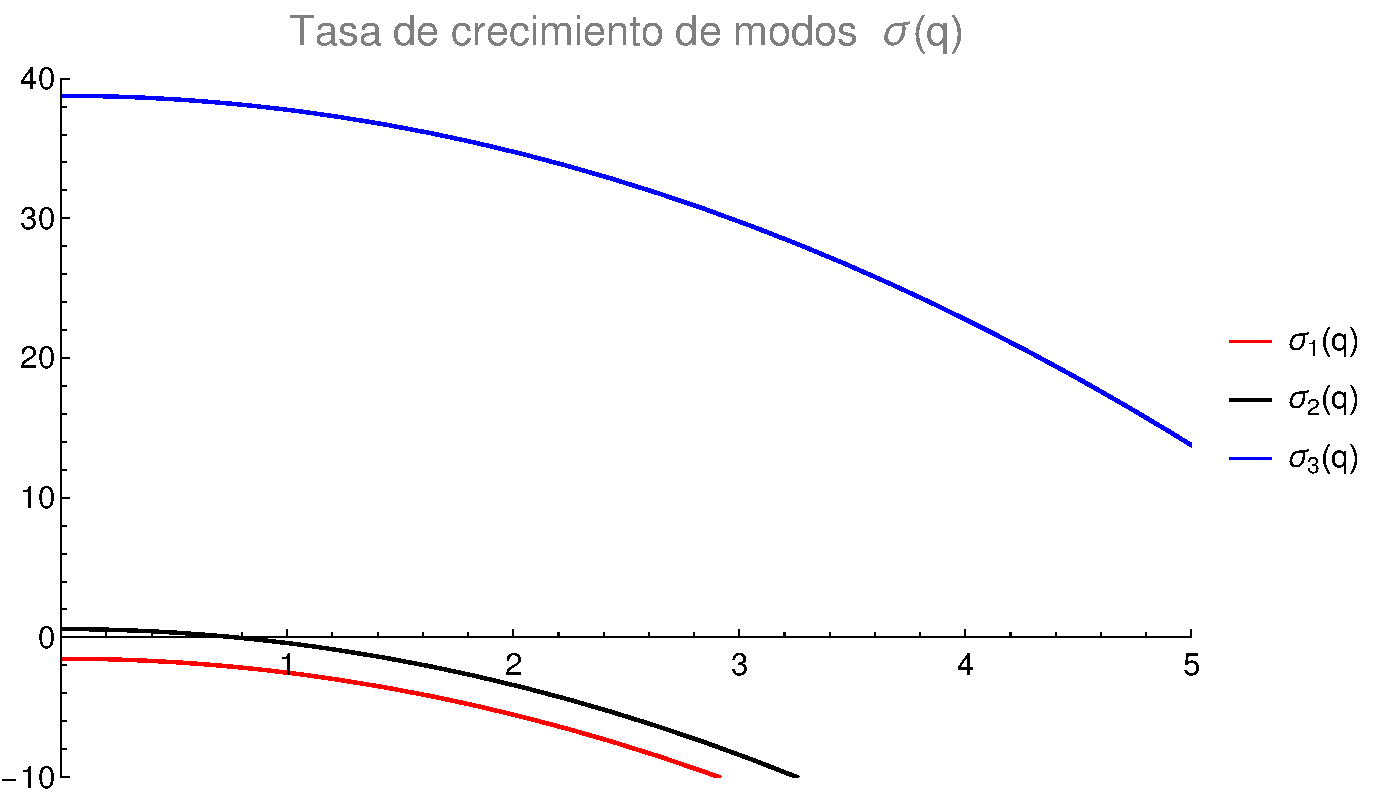
\includegraphics[width=0.6\textwidth]{images/estabilidad_p2.pdf}
    \caption{Estabilidad $P_2$}
    \label{fig:estabilidad_p2}
\end{figure}


\begin{figure}[ht]
    \centering
    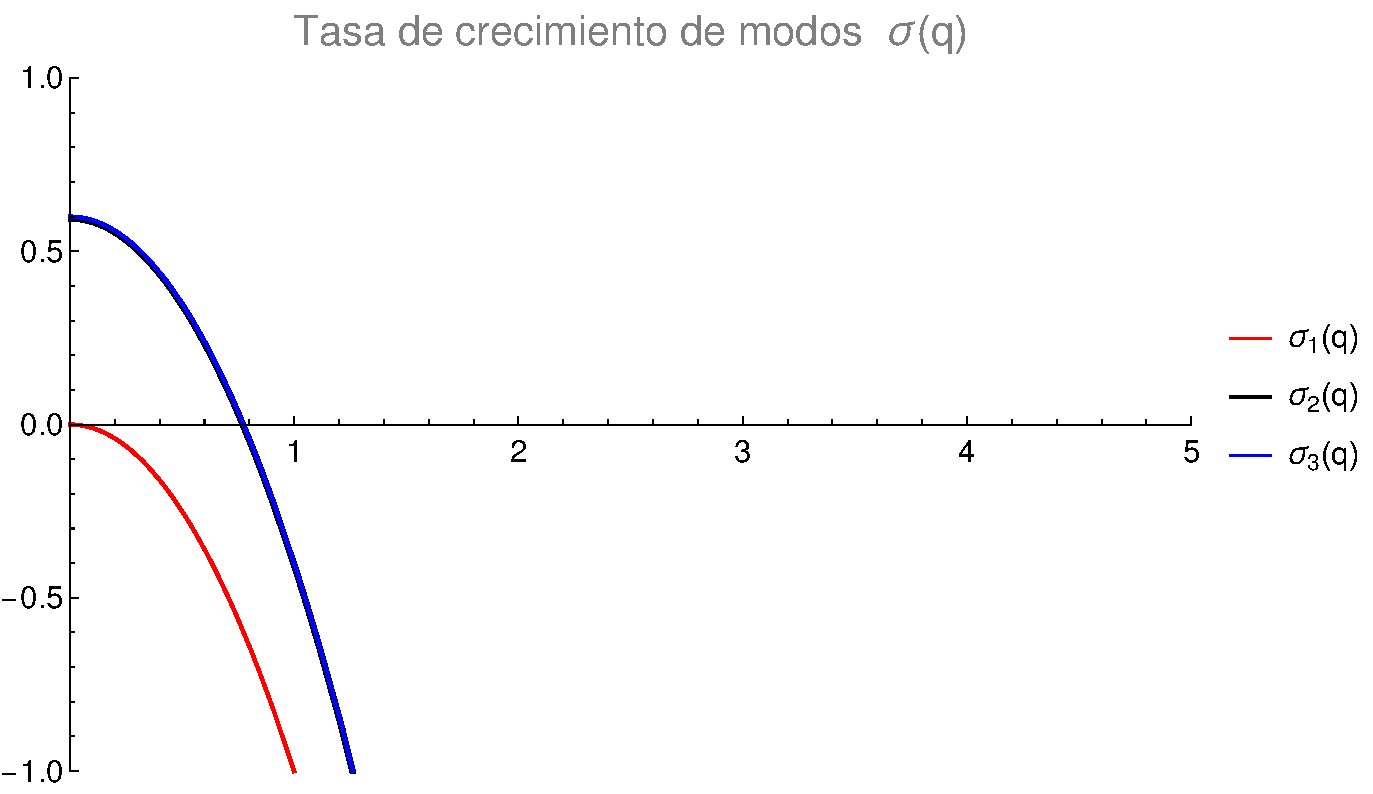
\includegraphics[width=0.6\textwidth]{images/estabilidad_p3.pdf}
    \caption{Estabilidad $P_3$}
    \label{fig:estabilidad_p3}
\end{figure}


\newpage
\bibliographystyle{alpha}
\bibliography{sample}

\end{document}